%\documentstyle[epsf,twocolumn]{jarticle}       %LaTeX2.09仕様
%\documentclass[twocolumn]{jarticle}     %pLaTeX2e仕様
\documentclass{jarticle}     %pLaTeX2e仕様

%一枚組だったら[twocolumn]関係のとこ消す

\setlength{\topmargin}{-45pt}
%\setlength{\oddsidemargin}{0cm} 
\setlength{\oddsidemargin}{-7.5mm}
%\setlength{\evensidemargin}{0cm} 
\setlength{\textheight}{24.1cm}
%setlength{\textheight}{25cm} 
\setlength{\textwidth}{17.4cm}
%\setlength{\textwidth}{172mm} 
\setlength{\columnsep}{11mm}

\kanjiskip=.07zw plus.5pt minus.5pt

\usepackage{graphicx}
\usepackage[dvipdfmx]{color}
\usepackage{subcaption}
\usepackage{enumerate}
\usepackage{comment}
\usepackage{url}
\usepackage{multirow}
\usepackage{diagbox}
\usepackage{float}

\begin{document}

  \noindent
  \onecolumn
  \hspace{1em}

  \today ゼミ
  \hfill
  \ \  B3 西村昭賢 

  \vspace{2mm}
  \hrule
  \begin{center}
  {\Large \bf 進捗報告}
  \end{center}
  \hrule
  \vspace{3mm}


\section{今週やったこと}

\begin{quote}
  \begin{itemize}
   \item 実験に用いるサンプルゲームの作成
   \item 実験環境および実験方法の検討
  \end{itemize}
 \end{quote}

\section{サンプルゲーム}
森先生から頂いたテーマに即して,実験で用いる自作のカードゲームを Unity を用いて作成した.
Windows10 を搭載した PC で作成し, 使用した Unity のバージョンは 2020.3.29f1 であった.\par
図 1 にゲームのプレイ画面を示す.


\begin{figure}[H]
  \centering
  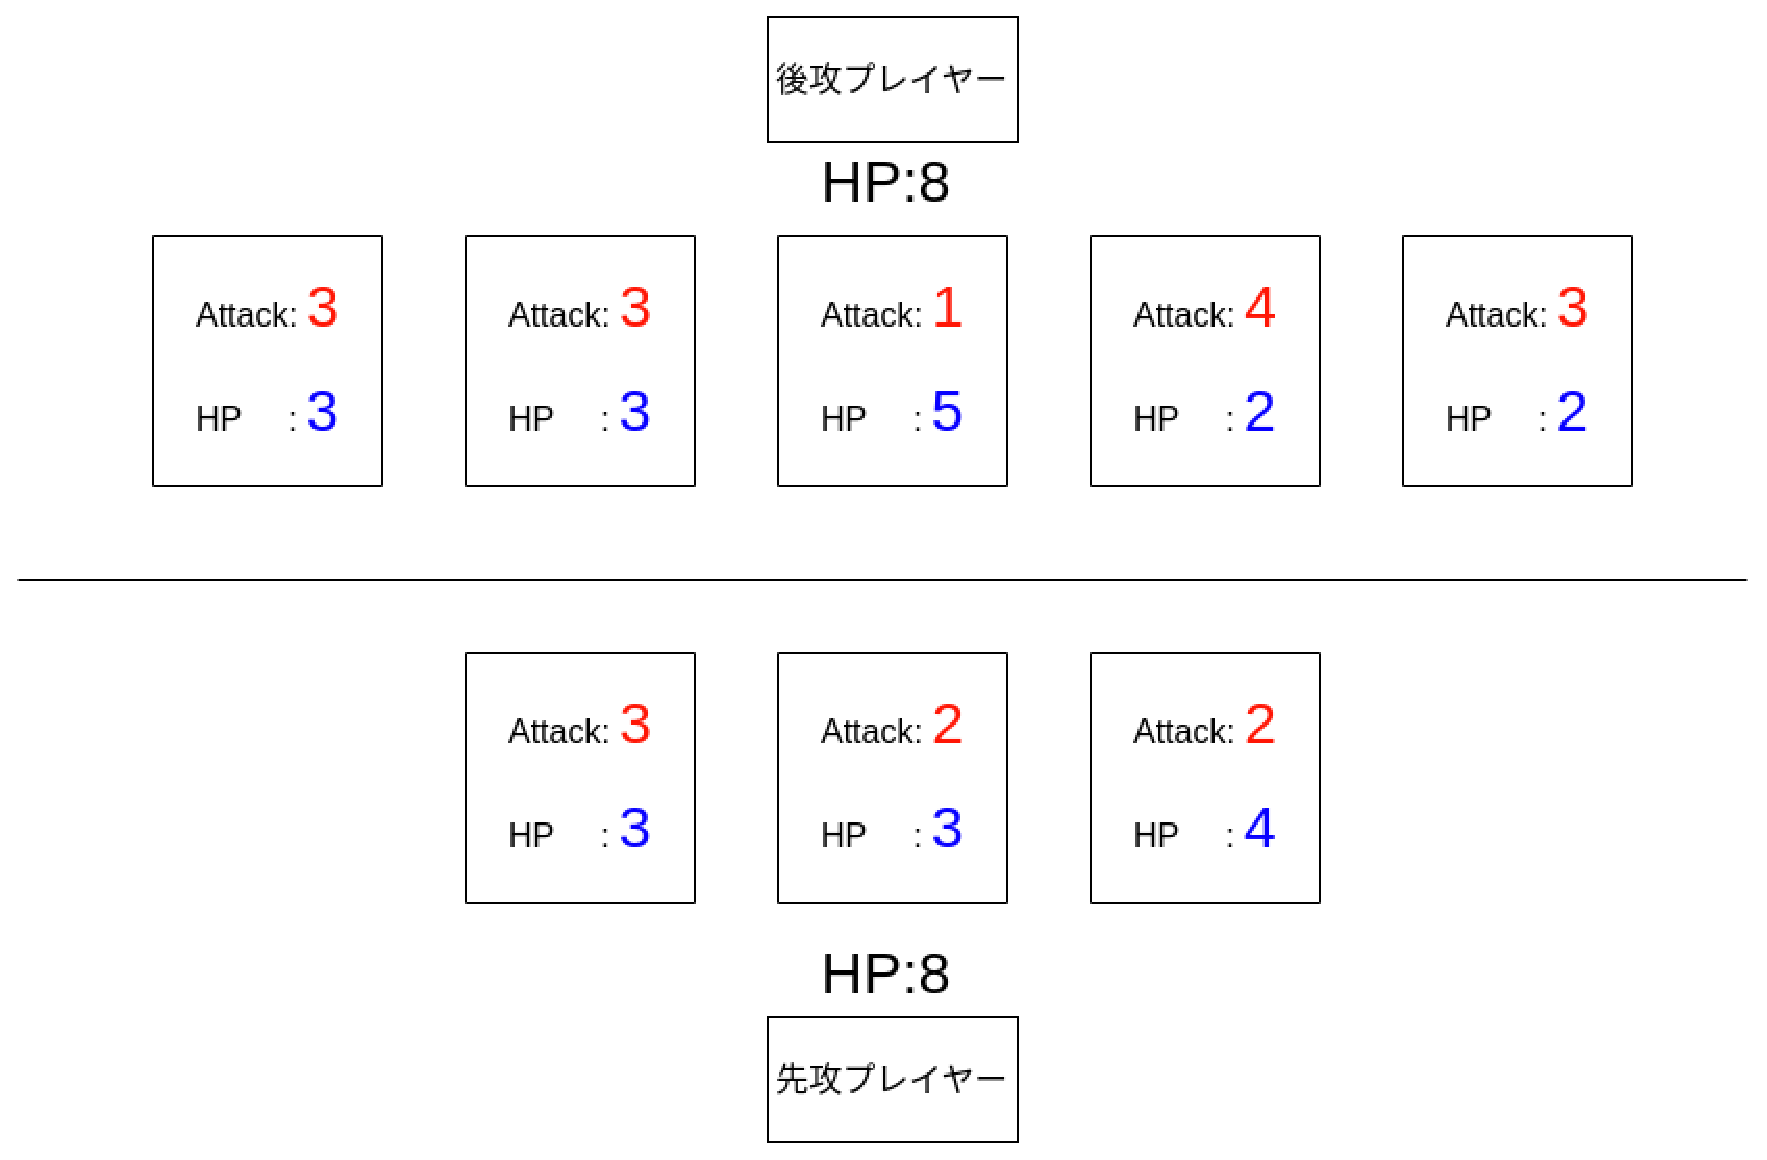
\includegraphics[width=160mm]{assets/Figure1.eps}
  \caption{作成したカードゲームのプレイ画面}
  \label{fig:sample}
\end{figure}

図\ref{fig:sample}において,画面上下部に存在する Player と Enemy がゲームの参加者である.
 Player , Enemy の右側に存在する赤丸は HP を表しておりこれを 0 にすることが本ゲームの勝利条件となる.
 左側に存在する緑丸はマナコストを表しカードを場に出すとこの数値はカードのコストに応じて減っていく.
画面右側の青色のボタンを押すとターンが代わり,ボタンの上の数字は Player , Enemy それぞれの持ち時間を示している.
ターン終了後にはマナコストは以前のターンより 1 つ多く回復する.
\begin{figure}[htbp]
  \centering
  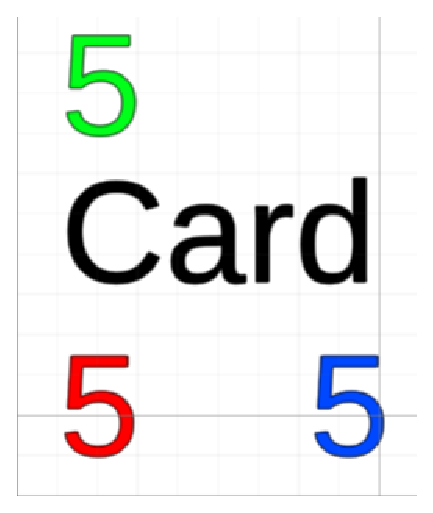
\includegraphics[width=60mm]{assets/Figure2.eps}
  \caption{カードのUI}
  \label{fig:card}
\end{figure}

図\ref{fig:card}に示すようにカードは3種類の数字を持つ.
図\ref{fig:card}において左下の赤い数字はカードの攻撃力を示す.また,右下の青い数字はカードの HP を示す.左上の緑色の数字はカードのコストを表す.
今回作成したゲームではその場に出た時にすぐ行動できるカード,自身が場に出た時は敵カードは自身以外に攻撃できないといった特殊効果を持つカードも実装している.
また一般的なカードゲームにおけるスペルカードも実装している.スペルカードは自身が場に出ない代わりに,使用すると何らかの効果を与えるカードである.
\par
\par
\par
今回実装したスペルの種類を以下に示す.
\begin{quote}
  \begin{itemize}
   \item 場に出ている敵カード 1 枚に一定数ダメージを与える.
   \item 場に出ている敵カード全てに一定数のダメージを与える.
   \item 敵に一定数のダメージを与える.
   \item 場に出ている味方カード 1 枚を一定数回復する.
   \item 場に出ている味方カード全てを一定数回復する.
   \item 自身を一定数回復する.
  \end{itemize}
 \end{quote}



\section{実験環境および実験方法の検討}
本研究テーマ「自作カードゲームの難易度調整AIの作成」に類似した研究を参考に,実験環境および実験方法の検討を行った.

\subsection{MCS-AI動的連携モデル}
ゲーム AI のモデルアーキテクチャとして,ゲーム全体を俯瞰的に認識しゲーム内のあらゆる要素をコントロールするメタ AI ,キャラクターの頭脳と身体を含めたキャラクター AI ,自律的に環境を解析し必要な情報を提供することでキャラクター AI とメタ AI をサポートするスパーシャル AI と大きく 3 つに分けそれらを相互に左右させる MCS-AI 動的連携モデルが考案されている\cite{MCSAIモデル}.


\subsection{MCS-AI動的連携モデルにおける類似研究}
宋,三宅らは MCS-AI 動的モデルを用いて,ゲームの難易度に関わるパラメータを unity 側が一定間隔で Python 側に送信し, Python 側で k 近傍法を用いてチューニング処理を行ったパラメータを Unity 側が反映するといった形で Unity で作成した FPS ゲームの難易度自動調整を試みた\cite{FPS}. \cite{FPS}の結果としてはチューニングが十分ではなく,改善が必要という結論に至ったが, 使用された図 \ref{fig:Unity} のUnity と Python の連携方法は本研究に活かせると考えた.

\begin{figure}[htbp]
  \centering
  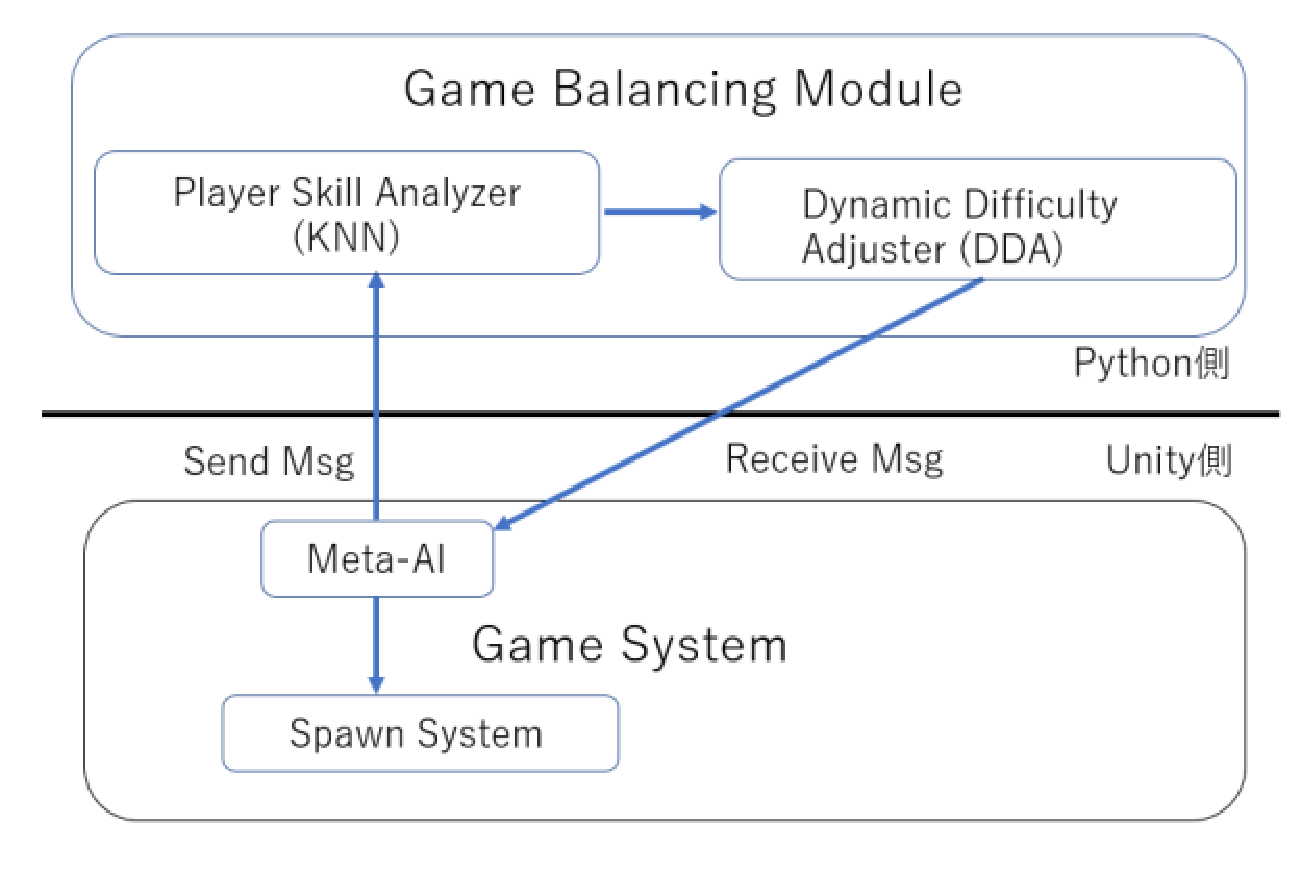
\includegraphics[width=110mm]{assets/Figure3.eps}
  \caption{FPS自動難易度調整の研究で用いられた Unity と Python の連携}
  \label{fig:Unity}
\end{figure}

\subsection{検討手法}
以上のことを踏まえ,本研究では図 \ref{fig:class図}のような実験環境を想定した.
PlayerAI と EnemyAI が対戦を行いそのログを Python側 へ送る. Python 側でそのログからパラメータのチューニングを行い, Unity 側に送り反映する.これを繰り返すといった形で実験できると考えた.

\subsection{試したこと}

\begin{quote}
  \begin{itemize}
   \item UbuntuへのUnityのインストール
   \par
   インストールと実行確認はしたが, Unity で強く推奨されている VisualStudio が使えなかったためコードを書く際に補完機能などが無く開発が難しい.
   \item Socket通信
   \par 
   ネット上のサンプルコード\cite{サンプルコード}を試した結果,研究室の PC の環境で Unity と Python 間の相互の socket 通信は正常に動作した.サンプルコードは Unity3D 用だったが作成した 2D のカードゲームに適用する作業が必要である.
  \end{itemize}
 \end{quote}



\begin{figure}[htbp]
  \centering
  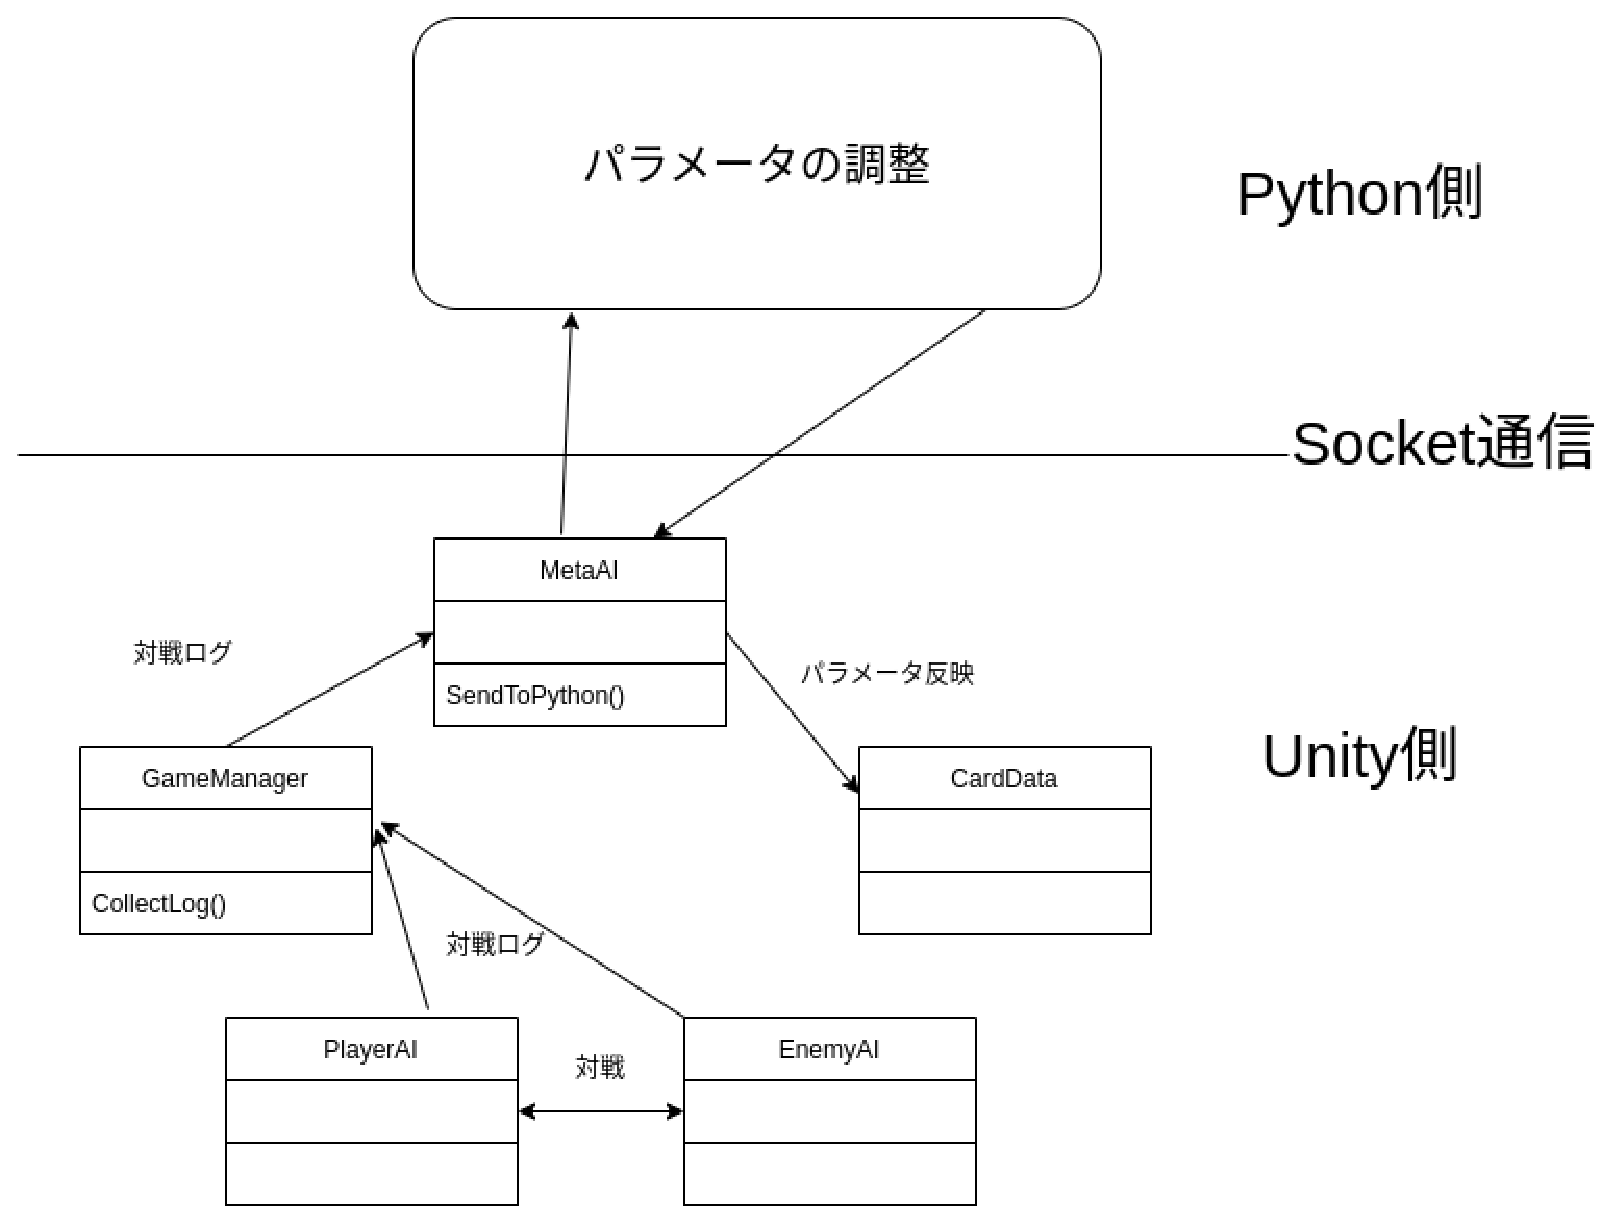
\includegraphics[width=140mm]{assets/Figure4.eps}
  \caption{本研究での実験環境案}
  \label{fig:class図}
\end{figure}



\section{今後やること}

\begin{quote}
  \begin{itemize}
    \item サンプルゲームの Ubuntu への移植
    \item サンプルゲームの改良(ログの生成,リファクタリング,Socket通信)
    \item Python 側の内部処理の方法の検討
    \item 調整するパラメータの選定, playerAI,enemyAIの動作といった実験条件の決定
  \end{itemize}
 \end{quote}



%index.bibはtexファイルと同階層に置く
%ちゃんと\citeしないと表示されない(1敗)
\bibliography{index.bib}
\bibliographystyle{junsrt}

\end{document}